\chapter{Communication Protocol}

Included pieces of code that may not be obvious to users or code that was particularly important to the operation of the protocol ...

%\inputminted{octave}{BitXorMatrix.m}

\begin{listing}[ht]
\begin{minted}[
linenos,
bgcolor=smokyblack]{c}
struct __attribute__((__packed__)) RXPacketStruct {
	uint8_t START[2];
	...
	uint8_t StatBIT_1 : 1; //Bit field
	uint8_t StatBIT_2 : 1;
	uint8_t StatBIT_3 : 1;
	...
	uint8_t CRCCheck[2]; //CRC-CCITT        
	uint8_t STOP[2];
};
\end{minted}
\caption{PC RX "packed" packet structure.}
\label{listing:packet-packet}
\end{listing}

\begin{listing}[ht]
\begin{minted}[
linenos,
bgcolor=smokyblack]{c}
union {
	uint32_t WORD;
	uint16_t HALFWORD;
	uint8_t BYTE[4];
} WORDtoBYTE;
\end{minted}
\caption{Byte conversion union.}
\label{listing:Byte conversion union}
\end{listing}

\begin{listing}[ht]
\begin{minted}[
linenos,
bgcolor=smokyblack]{c}
HAL_UART_Receive_DMA(&PC_UART, RXBufPC, sizeof(RXPacket));
if(xSemaphoreTake( PCRXHandle, portMAX_DELAY ) == pdTRUE) {
	rcvdCount = sizeof(RXPacket);
	START_INDEX = findBytes(RXBufPC, rcvdCount, 
	RXPacket.START, 2, 1);
	if(START_INDEX>=0) {
		memcpy(RXPacketPTR, &RXBufPC[START_INDEX], 		
		sizeof(RXPacket));
		RX_DATA_VALID = 0;

		WORDtoBYTE.BYTE[1] = RXPacket.CRCCheck[0];
		WORDtoBYTE.BYTE[0] = RXPacket.CRCCheck[1];
		CALC_CRC = crcCalc(&RXPacket.OPCODE, 0, PAYLOAD_RX, 0);
		
		//A useful tool when calculating and 
		//confirming CRC values of various types: 
		//https://www.lammertbies.nl/comm/info/crc-		
		//calculation.html

		if(WORDtoBYTE.HALFWORD==CALC_CRC) {
			RX_DATA_VALID = 1;
			... //Packet processing
\end{minted}
\caption{PC RX packet processing.}
\label{listing:PC RX packet processing}
\end{listing}

\begin{listing}[ht]
\begin{minted}[
linenos,
bgcolor=smokyblack]{c}
void BaseCommandCompile(uint8_t n, uint8_t SeqBits, uint8_t ComBits, 
uint8_t INDOFF1, uint8_t INDOFF2, uint8_t *DATA, 
uint8_t LEN, uint8_t SNIP);
\end{minted}
\caption{Motor packet compilation function.}
\label{listing:Motor packet compilation function}
\end{listing}

\begin{listing}[ht]
\begin{minted}[
linenos,
bgcolor=smokyblack]{c}
BaseCommandPTR = &BaseCommand[RXPacket.OPCODE];
BaseCommandCompile(RXPacket.OPCODE, 0b0011, 0x02, 0x45, 0x02,
RXPacket.M1C, 2, 0);
xQueueOverwrite(ICommandM1QHandle, &BaseCommandPTR);
\end{minted}
\caption{Motor packet compilation current command example.}
\label{listing:Motor packet compilation example}
\end{listing}

\begin{figure}
\centering
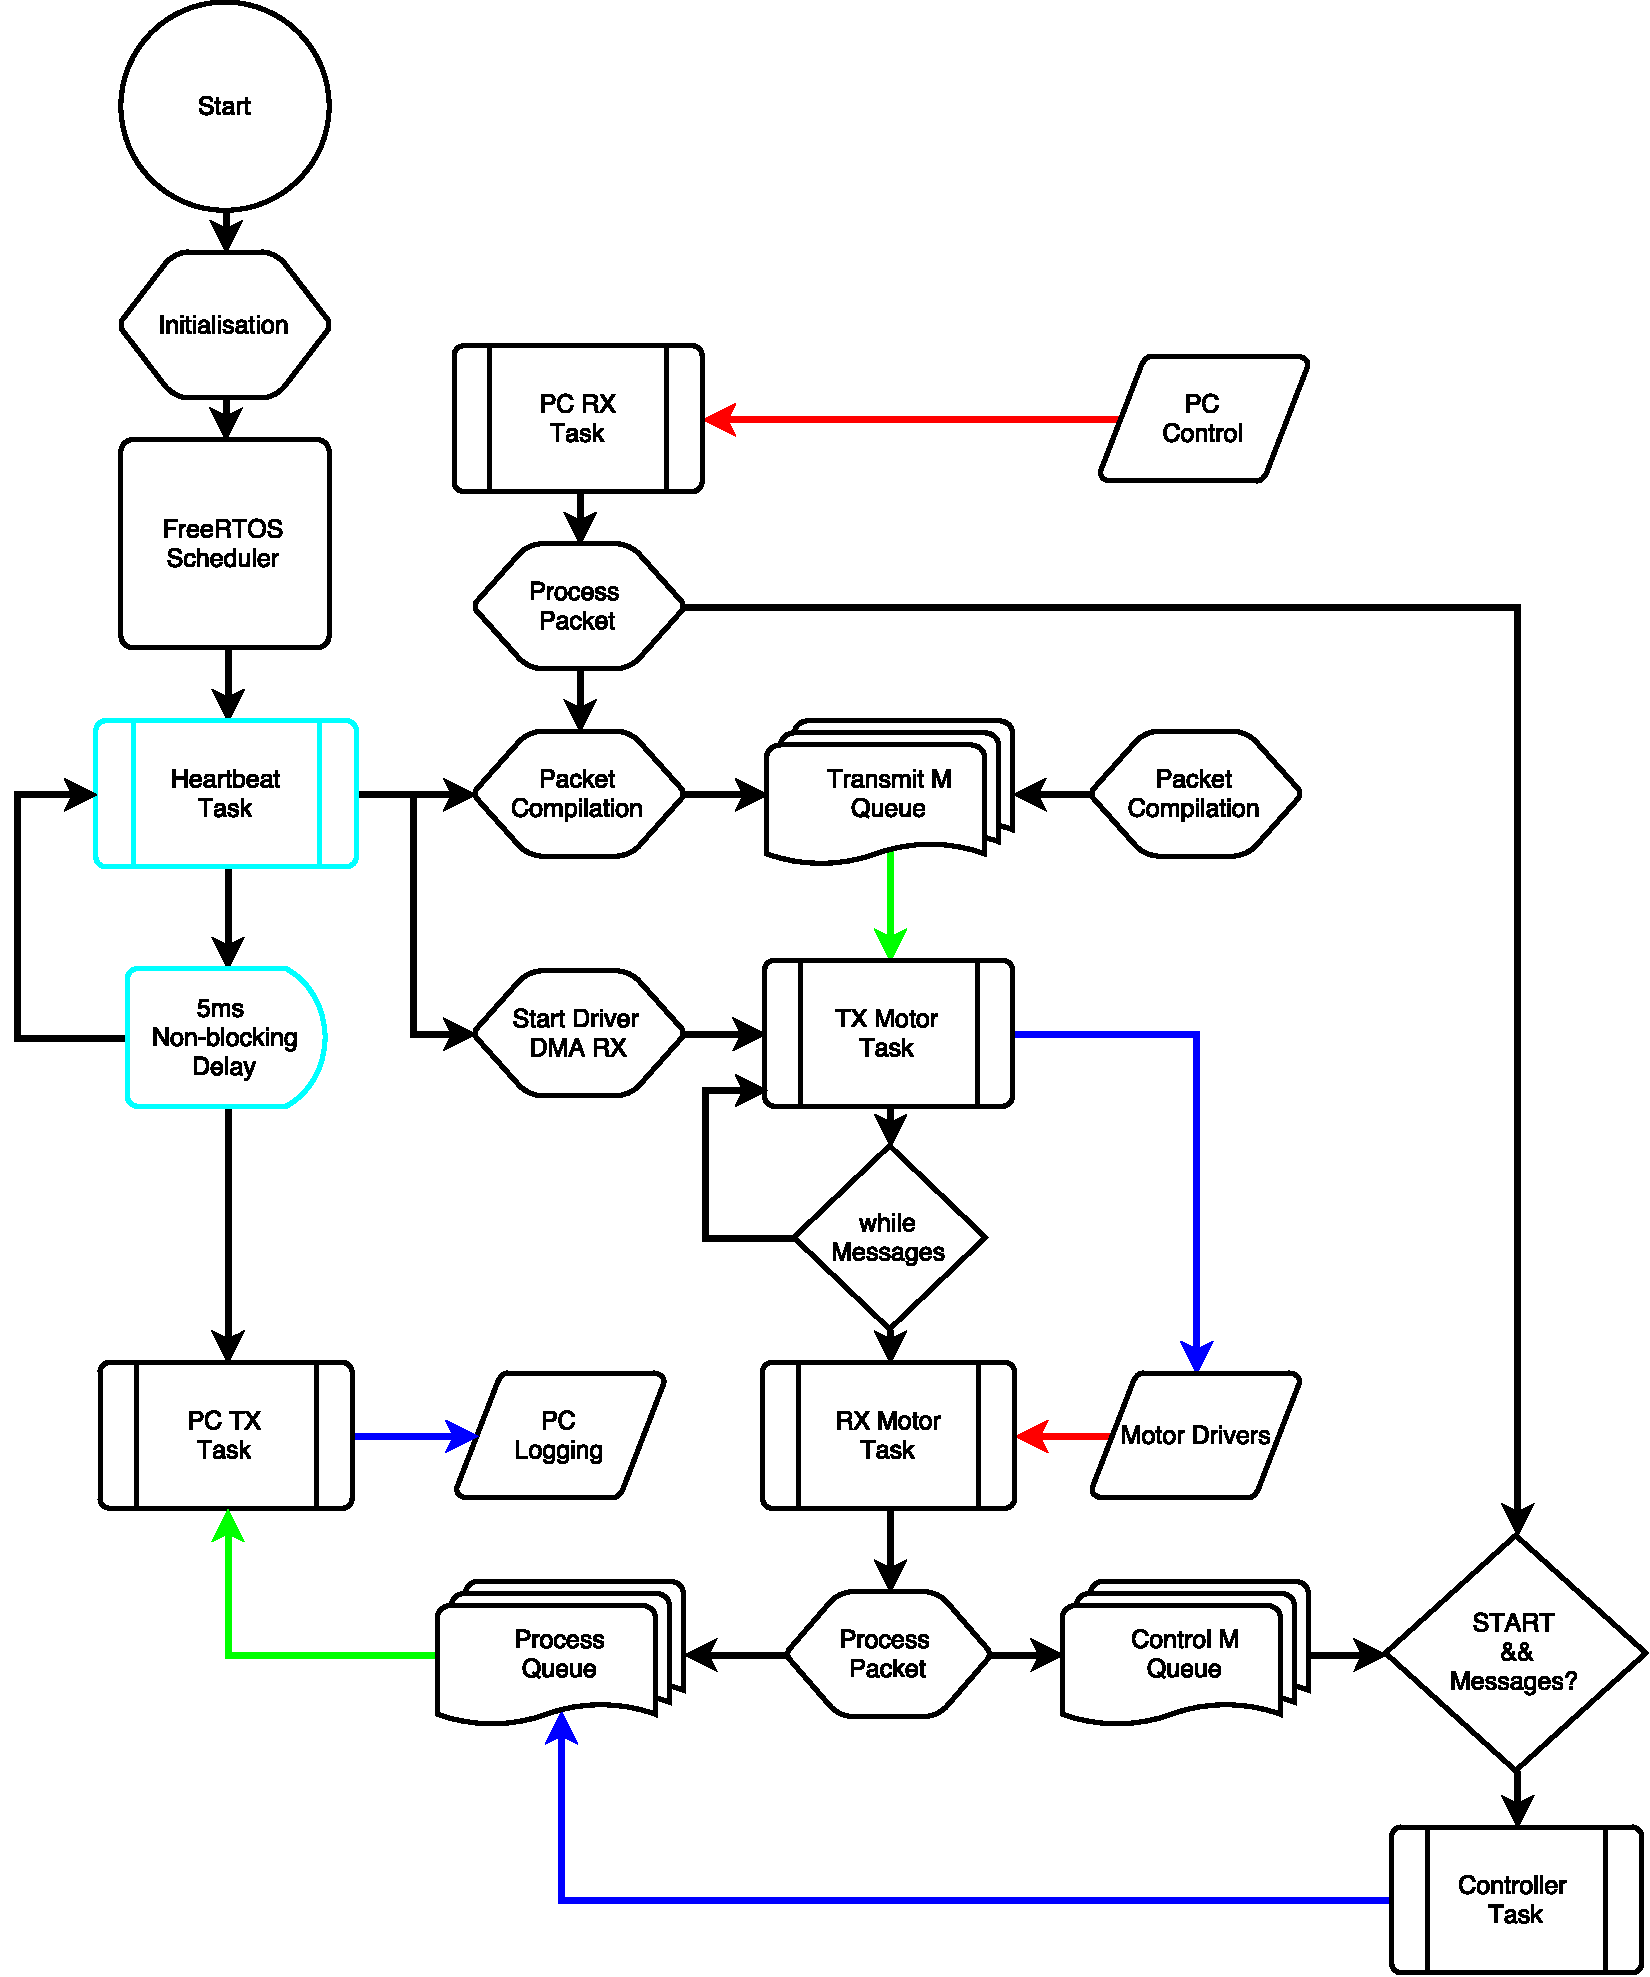
\includegraphics[width=1\textwidth]{images/comms/communication-flow-diagram.pdf} 
\caption{FreeRTOS communication protocol flow diagram.}
\label{fig:FreeRTOS communication protocol flow diagram.}
\end{figure}

\begin{figure}
\centering
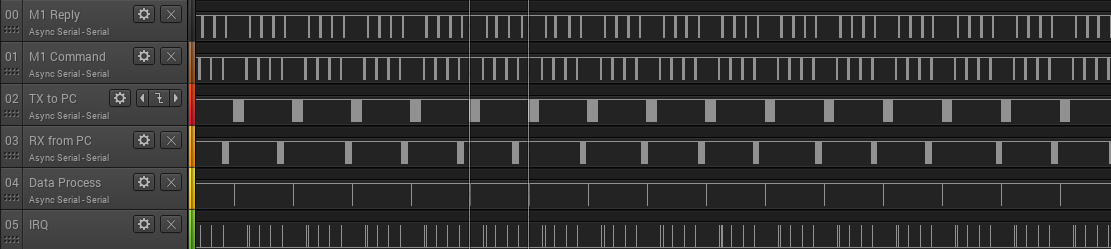
\includegraphics[width=1\textwidth]{images/comms/pc-packet-timing-data} 
\caption{Communication protocol packet timing with 5 ms sampling rate.}
\label{fig:packet-timing.}
\end{figure}

\begin{table}
\centering
\begin{tabular}{llllll}
\textbf{Command}       & \textbf{Index} & \textbf{Op-Code} & \textbf{TX CB} & \textbf{TX CRC1} & \textbf{RX  CB} \\
\textbf{Kill Bridge}   & 1              & 0001             & 0x06           & 0xCBB6           & 0x04            \\
\textbf{Write Enable}  & 2              & 0010             & 0x0A           & 0x3624           & 0x08            \\
\textbf{Bridge Enable} & 3              & 0100             & 0x12           & 0x1AE0           & 0x10            \\
\textbf{Set Current}   & 4              & 0011             & 0x0E           & 0xBF7B           & 0x0C            \\
\textbf{Read Current}  & 5              & 1100             & 0x31           & 0x9772           & 0x32            \\
\textbf{Read Position} & 6              & 1111             & 0x3D           & 0xD310           & 0x3E            \\
\textbf{Read Velocity} & 7              & 0101             & 0x15           & 0x5EAF           & 0x16            \\
\textbf{Set Position}  & 8              & 1010             & 0x2A           & 0x42C4           & 0x28           
\end{tabular}
\caption{Motor driver command protocol.}
\label{tab:motor-driver-protocol}
\end{table}